\documentclass{article}

\usepackage{booktabs} 
\usepackage[english]{babel}
\usepackage{graphicx}
\usepackage{amsmath}

\title{Review questions linear regression}
\date{14-09-2016}
\author{Wendy Nieuwkamer}

\begin{document}

\maketitle

\section{Question 6}
Apply gradient descent by hand onthe training set given in Table 1.

\begin{figure}[h!]
    \center
    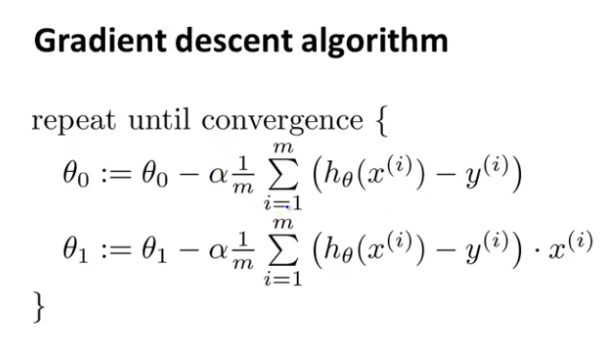
\includegraphics[scale=0.4]{Gradient_descent_algorithm}
    \label{GDA}
\end{figure}


Hypothesis:
\begin{equation}
h_{\theta}(x^{(i)}) = \theta _0 + \theta _1 x^{(i)}
\end{equation}

\begin{table}[h!]
  \centering
  \caption{Training examples}
  \label{tab:table1}
  \begin{tabular}{cc}
    \toprule
    x & y \\
    \midrule
    3&2\\
    1&2\\
    0&1\\
    4&3\\
    \bottomrule
  \end{tabular}
\end{table}

We have four training examples, so $m=4$. Let's take $\alpha = 0.1$. And start values $\theta _0 = -1.0$  and $\theta _1 = 0.5$. First, do the calculations as seen in equations 2 to 9.

\begin{align}
    \theta _0 &= \theta _0 - \alpha \frac{1}{4} \sum\limits_{i=1}^4 (h _{\theta} (x ^{(i)}) - y ^{(i)}) \\
    &= -1.0 - 0.1 \cdot \frac{1}{4} \cdot (-1.5 - 2.5 - 2 -2 )\\
    &= -1.0 - 0.1 \cdot  0.25 \cdot -8\\
    &= -0.8\\
    \theta _1 &= \theta _1 - \alpha \frac{1}{4} \sum\limits_{i=1}^4 (h _{\theta} (x ^{(i)}) - y ^{(i)})x^{(i)} \\
    &=0.5 - 0.1 \cdot \frac{1}{4} \cdot (-4.5 -2.5 + 0 - 8) \\
    &= 0.5 - 0.1 \cdot 0.25 \cdot -15 \\
    &=0.875
\end{align}

Then, assign the new values to $\theta$; $\theta _0 = -0.8$ and $\theta _1 = 0.875$. Repeat this process until it starts to converge or diverge. In the latter case choose $\alpha$ smaller. Otherwise, you have approached the optimal values for $\theta _0$  and $\theta _1$. The best way to decide wether you are close to the optimum is by looking at the gradient. If this approaches zero it means you are approaching the optimum.


\end{document}